\documentclass[12pt]{report}

\usepackage[utf8]{inputenc}
\usepackage{t1enc}
\usepackage[magyar]{babel}
\usepackage{amsmath}
\usepackage{url}
\usepackage{graphicx}

\graphicspath{ {./latex_images} }

\newcommand*{\xdash}[1][3em]{\rule[0.5ex]{#1}{0.55pt}}
\newcommand*{\ydash}[1][0.9em]{\rule{0.55pt}{#1}}


\title{Structure from Motion from Two Views}
\date{}

\begin{document}
    \maketitle

    \chapter{Algoritmus}
    A Structure from motion (SfM) folyamat segítségével 3D rekonstrukciót hajthatunk végre egy képpár segítségével.

    \begin{enumerate}
        \item Két kép közötti ritka ponthalmazok megfeleltetése (pontmegfeleltetés): az első kép sarokpontjainak azonosítása a \textit{detectMinEigenFeatures} függvénnyel, majd azok követése a második képre a \textit{vision.PointTracker} segítségével.
        \item Az esszenciális mátrix becslése \textit{estimateEssentialMatrix} használatával.
        \item Kamera elmozdulásának kiszámítása \textit{estrelpose} függvénnyel.
        \item Két kép közötti sűrű ponthalmazok megfeleltetése (pontmegfeleltetés): több pont kinyeréséhez újra kell detektálni a pontokat a \textit{detectMinEigenFeatures} függvény segítségével a \textit{'MinQuality'} opciót használva. Ezt követi a sűrű ponthalmaz követése a második képre a \textit{vision.PointTracker} használatával.
        \item Az illeszkedő pontok 3D helyzeteinek meghatározása a \textit{triangulate} segítségével (háromszögelés).
    \end{enumerate}    

    \chapter{Kód magyarázata}
        \section{Képpár betöltése}
            \begin{enumerate}
                \item \textit{fullfile(string1, string2, ...)} = az argumentumként kapott stringekből összeállít egy elérési útvonalat, pl.:\\\\
                    \texttt{path = fullfile('myfolder', 'mysubfolder')\\path = 'myfolder\textbackslash mysubfolder\textbackslash '}\\\\
                    \textit{toolboxdir(toolbox)} = visszaadja az argumentumként kapott toolbox abszolút elérési útvonalát.
                \item \textit{imageDatastore(path)} = létrehoz egy ImageDatastore objektumot a kapott elérési útvonallal meghatározott képekből. Az ImageDatastore objektum segítségével egy mappában található összes képet össze lehet gyűjteni egy változóba (de alapból nem lesz az összes kép egyszerre betöltve).
                \item \textit{readimage(datastore, n)} = betölti az n. képet a megadott datastore-ból.
                \item \textit{figure} = létrehoz egy új, üres ábra ablakot.
                \item \textit{imshowpair(image1, image2, 'montage')} = a meghatározott két képet egymás mellé helyezi a legutolsó ábrán.
                \item \textit{title('string')} = hozzáad egy címet a legutolsó ábrához.
            \end{enumerate}

        \section{A Camera Calibrator alkalmazás segítségével előre kiszámolt kamera paraméterek betöltése.}
            \begin{enumerate}
                    \item \textit{load(file\_name.mat)} = betölti egy korábban elmentett workspace adatait a jelenlegi workspace-be. A workspace egy ideiglenes tároló amely a MATLAB elindítása óta létrehozott változókat tárolja. Alapértelmezetten a MATLAB ablak jobb oldalán látható. A workspace-t el lehet menteni, így a benne tárolt változókat később vissza lehet tölteni a MATLAB-ba.
            \end{enumerate}

        \section{Lencse által okozott torzítás eltávolítása.}
            \begin{enumerate}
                \item \textit{undistortImage(image, intrinsics)} = a második argumentumként megadott kamera paramétereket felhasználva eltűnteti a kamera lencséje által okozott torzítást a megadott képről.\\
                      A kamera kalibrációja során kapott kamera paramétereket és a torzítási együtthatókat felhasználva kiszámítjuk a bemeneti kép minden pixelének eredeti pozícióját. Az egyes pixelek pozícióját az alábbi torzítások módosítják:
                        \begin{itemize}
                            \item \textbf{Radiális torzítás} = kiváltó oka, hogy a lencse szélén áthaladó fény jobban törik, mint a lencse közepén környezetében áthaladó fény. Ez kiszámolható:\\
                                \[x_r = x(1 + k_1r^2 + k_2r^4)\]
                                \[y_r = y(1 + k_1r^2 + k_2r^4)\]
                                (Ahol $x_r, y_r$ = radiális torzulásmentes koordináták; $x, y$ = torzított koordináták; $k_1, k_2$ = radiális torzítási együtthatók; $r^2 = x^2 + y^2$)
                            \item \textbf{Tangenciális fordítás} = előfordul, ha a kameraszenzor és a lencse nem állnak tökéletesen párhuzamosan. Ez kiszámolható:\\
                                \[x_t = 2p_1xy + p_2(r^2+2x^2)\]
                                \[y_t = 2p_2xy + p_1(r^2 + 2y^2)\]
                                (Ahol $x_t, y_t$ = tangenciális torzulásmentes koordináták; $x, y$ = torzított koordináták; $p_1, p_2$ = tangenciális torzítási együtthatók; $r^2 = x^2 + y^2$)\\\\
                                A végső együttható értékének kiszámítása:
                                \[x_f = x_r + x_t\]
                                \[y_f = y_r + y_t\]
                    Az egyes pixelek korrigált helyének kiszámítása nem egész számú értékeket is előállít. Mivel a nem egész szám nem lehet pixel koordináta, ezért bilineáris interpolációt is végre kell hajtani. A bilineáris interpoláció során, a legközelebbi négy szomszédot felhasználva először lineáris interpolációt hajtunk végre az egyik irányba (pl. az x tengely mentén), majd pedig a másik irányba (az y tengely mentén):
                        \[out_P = I_1(1 - \Delta X)(1 - \Delta Y) + I_2 (\Delta X)(1 - \Delta Y) + I_3(1 - \Delta X)(\Delta Y) + I_4(\Delta X)(\Delta Y)\]
                        (Ahol $I_1, I_2, I_3, I_4$ = a szomszédos négy koordináta intenzitása az eredeti, torzított képen; $\Delta X, \Delta Y$ = a nem egész értékű koordinátákkal rendelkező vizsgált pixel és a vizsgált pixelhez legközelebb eső, egész értékű koordinátákkal rendelkező szomszédai közötti távolság; $out_P$ = végeredményként kapott pixel intenzitás)\\\\
                    A szomszédos pixelek efféle súlyzott átlagolásával, az interpoláció eredményeképp egy pixel intenzitás értéket kapunk, amely a legközelebbi egész érték koordinátával rendelkező pixel intenzitása lesz.\\
                    Az előállított, torzítatlan képen néhány pixel (leginkább a kép szélein) nem rendelkezik megfelelő pixel párral az eredeti, torzított képről (ezek azok a területek, ahol az eredeti képből nincs információ). Ezek a pixelek alapértelmezetten 0 értéket kapnak (feketék lesznek). 
                        \end{itemize}
                \end{enumerate}

            \section{Pontmegfeleltetés a képek között.}
                \begin{enumerate}
                    \item \textit{detectSIFTFeatures(grayImage, ContrastThreshold=0.03)} = a SIFT (Scale-Invariant Feature Transform), vagyis a méretfüggetlen jellemző transzformáció algoritmus segítségével keres jellemzőpontokat.\\
                        A Shi és Tomasi féle minimum sajátérték algoritmus forgatásfüggetlen (ugyanis az elforgatott sarokpont megtartsa a sarokpont tulajdonságait), viszont nem skála-invariáns (invariáns = független) (pl.: ha egy fix ablakméretet használunk miközben a képet kicsinyítsük [elméletben nagy méretű nagyítás esetén is érvényes], akkor a sarokpont "kisímultnak" tűnhet).\\
                        \includegraphics[scale=0.8]{small_big_window_diff.png}
                        A képből látszik, hogy kicsi ablakméretet használva a sarkot inkább egy élnek, mint saroknak detektálnánk, míg nagy ablakméret esetén a sarkosság egyértelmű.\\
                        A SIFT lépései:\\
                            \begin{enumerate}
                                \item \textbf{Gauss-skálatér előállítása}. Ehhez ismét egy képpiramis-szerűséget hozunk létre. Az első szinthez az eredeti \textit{I(x,y)} képen különböző erősségű Gauss szűrőket alkalmazunk. Így kapunk egy kép kupacot, amelyen az egyik irányba haladva, az eredeti kép egyre inkább elmosódott példányait kapjuk. Ez az első szintet az első oktávnak (\textit{octave}) hívják. A következő szinthez, azaz a második oktávhoz az eredeti kép méretét a felére csökkentsük, és ezen ugyanúgy elvégezzük a különböző mértékű elmosásokat. Így hozunk létre több oktávot (az oktávok számát a kép eredeti felbontása határozza meg), amelyek a piramis szintjeit alkotják.\\
                                    \[L(x,y,\sigma) = G(x,y,\sigma) * I(x,y)\]
                                    ahol $G$ a Gauss függvény, amely meghatározza a $\sigma$ mértékű elmosódást:
                                    \[G(x,y,\sigma) = {1\over2\pi \sigma ^2}e^{-(x^2+y^2)/2\sigma^2}\]
                                    Miután elkészült a képpiramis, az egyes oktávokon belül található, különböző mértékben elmosott képeket kivonjuk egymásból (\textit{Difference of Gaussian}):\\
                                    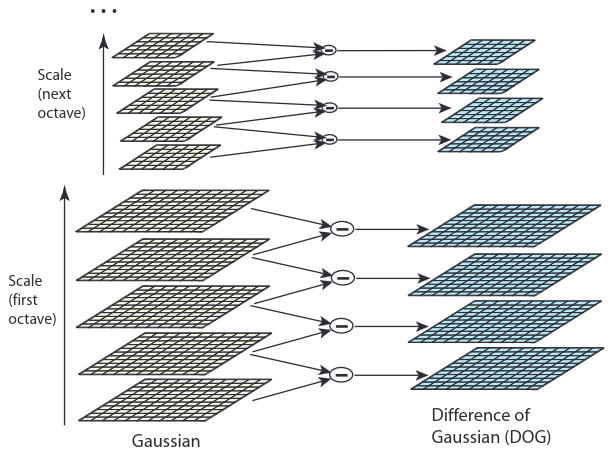
\includegraphics[scale=0.5]{DOG.png}
                                    \[D(x,y,\sigma) = L(x,y,k\sigma) - L(x,y,\sigma)\]
                                    ahol az egyes L értékek a különböző mértékben elmosott képek.
                                    Az így kapott képeken lokális szélsőértékeket keresünk pixelszomszédságok vizsgálatával. A vizsgált pixelt összehasonlítsuk a saját szintjén található 8 közvetlen szomszédjával, valamint az alatta és felette lévő szinteken található  9-9 szomszédos pixellel. Ha az adott pixel intenzitása nagyobb vagy kisebb, mint a 26 szomszédjáé, akkor a vizsgált pixel szélsőérték és egyben potenciális kulcspont.\\
                                    \begin{center}
                                        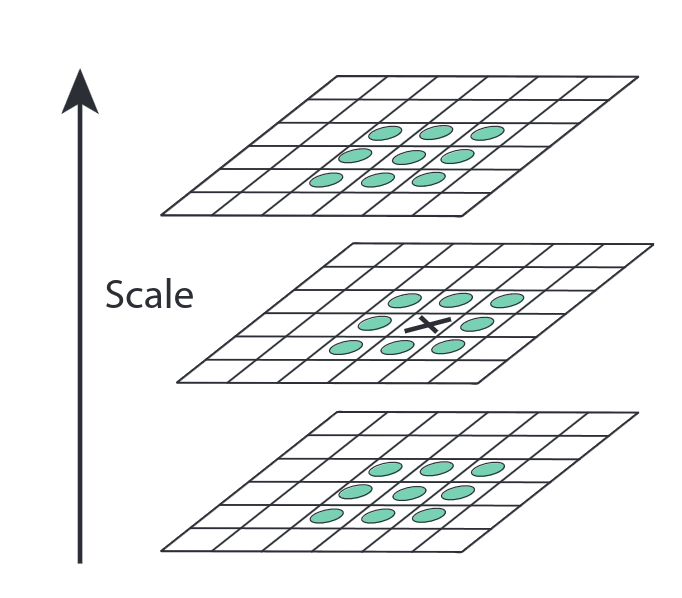
\includegraphics[scale=0.3]{extrema_check.png}
                                    \end{center}
                                    Következő lépésben Taylor-sort alkalmazva pontosítsuk a szélsőértékek pozícióját. A potenciális kulcspontok között vannak gyenge kontrasztú pontok. A gyenge kontrasztú pontok nem elég stabilak, nem zajállóak, nehezen megkülönböztetheőek, vagy akár maguk is zajok lehetnek. Emiatt, ha egy pont intenzitása nem éri el az előre meghatározott kontraszt küszöbértéket, akkor eldobjuk. A következő nem stabil pontok amelyeket ki kell szűrnünk azok az élek. Az élek kiszűréséhez 2x2 ún. Hess mátrixot (\textit{H}) használnak, melynek a sajátértékeinek az aránya mondja meg, hogy a vizsgált kulcspont egy él-e vagy sem. Ha ez az arány nagyobb, mint az előre meghatározott él küszöbérték, akkor a vizsgált kulcspont valószínűleg élhez tartozik, emiatt eldobjuk.
                                        \[H = \begin{bmatrix} D_{xx} D_{xy} \\ D_{xy} D_{yy} \end{bmatrix}\]
                                        \[Tr(H) = D_{xx} + D_{yy} = \alpha + \beta\]
                                        \[Det(H) = D_{xx}D_{yy} - (D_{xy})^2 = \alpha\beta\]
                                    ahol:
                                    \begin{itemize}
                                        \item $\alpha$ = a H mátrix nagyobb sajátértéke
                                        \item $\beta$ = a H mátrix kisebb sajátértéke
                                        \item $Tr(H)$ = a H mátrix nyoma
                                        \item $Det(H)$ = a H mátrix determinánsa
                                    \end{itemize}
                                    Legyen \textit{r} az arány $\alpha$ és $\beta$ között: $\alpha = r\beta$. Ekkor:
                                    \[{Tr(H)^2\over{Det(H)}} = {(\alpha + \beta)^2\over{\alpha\beta}} = {(r\beta + \beta)^2\over{r\beta^2}} = {(r + 1)^2\over{r}}\]
                                    ${(r + 1)^2\over{r}}$ minimum, ha a két sajátérték megegyezik (tehát \textit{r} = 1), és az \textit{r} értékkel együtt növekszik. Ebből megállapíthatjuk, hogy a két sajátérték aránya egy bizonyos küszöbérték ($r$) alatt van-e:
                                    \[{Tr(H)^2\over{Det(H)}} < {(r + 1)^2\over{r}}\]

                                \item \textbf{Orientáció hozzárendelése}. Mikor kulcsopontokat találtunk az első lépésben, azt is megtudtuk, hogy melyik skálaszinten találhatóak ezek a pontok, azaz tudjuk a skálázásukat, emiatt a kulcspontjaink skálainvariánsok. A következő lépés, a kulcspontok orientációjainak a kiszámítása, hogy a pontjaink forgatás invariánsok is legyenek. Ehhez a kulcspontok skálázásukkal arányos régióin belül minden pixelnél gradiens nagyságot és irányt számolunk:
                                            \[m(x,y) = \sqrt{(L(x+1,y) - L(x-1,y))^2 + (L(x,y+1) - L(x,y-1))^2}\]
                                            \[\theta(x,y)=tan^{-1}\left({(L(x,y+1) - L(x,y-1))\over{(L(x+1,y) - L(x-1,y))}}\right)\]
                                    ahol:
                                    \begin{itemize}
                                        \item $m(x,y)$ = gradiens nagysága
                                        \item $\theta(x,y)$ = gradiens iránya
                                        \item $L(x,y)$ = a Gauss-simítással kapott pixelintenzitás az adott pozícióban
                                    \end{itemize}
                                    Ezeket a kulcspont körüli pixelorientációkat egy orientációs hisztogramba rendezzük. Ez a hisztogram 36 csoportból áll, ahol minden csoport a 360 fokos térből egy 10 fokos szögtartományt képvisel. A pixelorientációk gradiens nagyságukkal és egy Gauss súlyozással ($\sigma$ = 1.5 x kép skála) súlyozva kerülnek az irányuknak megfelelő hisztogramtartományba (így mindegyik pixelorientáció a nagyságával és a kulcsponthoz való közelségével lesz súlyozva). Pl.: ha egy pixelorientáció 18.6 fokos, akkor a 10-19 tartományba fog kerülni:
                                    \begin{center}
                                        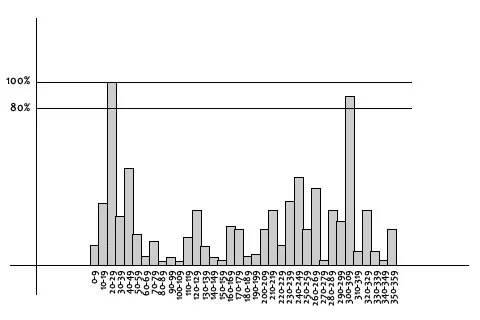
\includegraphics[scale=0.7]{orientation_histogram.png}
                                    \end{center}
                                    A hisztogramból kiválasztjuk a legnagyobb értékű tartományt és ennek a tartománynak a középpontja lesz a kulcspont domináns iránya. Ha a hisztogramban több csúcs is található amelyek nagysága egy bizonyos küszöbértéken belül van a fő csúcshoz képest (pl.: a fenti képen 80\%), akkor létrehozunk egy új kulcspontot az adott orientációval. Tehát ugyanazon pozícióval és skálázással jelenlévő kulcspontjaink is lehetnek, amelyek csak az irányukban különböznek. Ezen lépés után az összes jellemzőponthoz tartozni fog pozíció, skála, irány és magnitúdó.
                                \item \textbf{Kulcspont leíró készítése}. A leíró az egy olyan vektor, amely a kulcspont környezetét úgy írja le, hogy az a lehető legmegkülönböztethetőbb legyen, miközben invariáns a nézőpont- és megvilágításváltozásokkal szemben. Ehhez a kulcspont körüli 16x16-os méretű régiót vizsgáljuk, amit felosztunk 16db 4x4-es alrégiókra:\\
                                    \begin{center}
                                        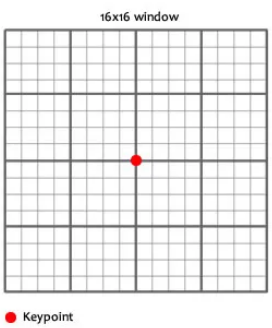
\includegraphics[scale=0.6]{descriptor_region.png}
                                    \end{center}
                                    A 4x4-es cellákon belül Gauss súlyozással (a cellák távolságával arányos súlyozást kapnak; $\sigma$ = leíró ablak szélességének a fele) kiszámítjuk az egyes pixelek gradiensének nagyságát és irányát (forgatás invariancia elérésehez a leíró koordinátáit és a gradiens orientációt a kulcspont orientációhoz relatívan elforgatjuk: mindegyik gradiens orientációból kivonjuk a kulcspont orientációját, így mindegyik gradiens orientáció a kulcspont orientációjához relatívan lesz megadva), amelyekből ismét létrehozunk egy orientációs hisztogramot. Minden irány/nyíl nagysága/hossza a régióban az adott irányhoz közel eső gradiens-magnitúdók összegét jelzi. \\
                                    \begin{center}
                                        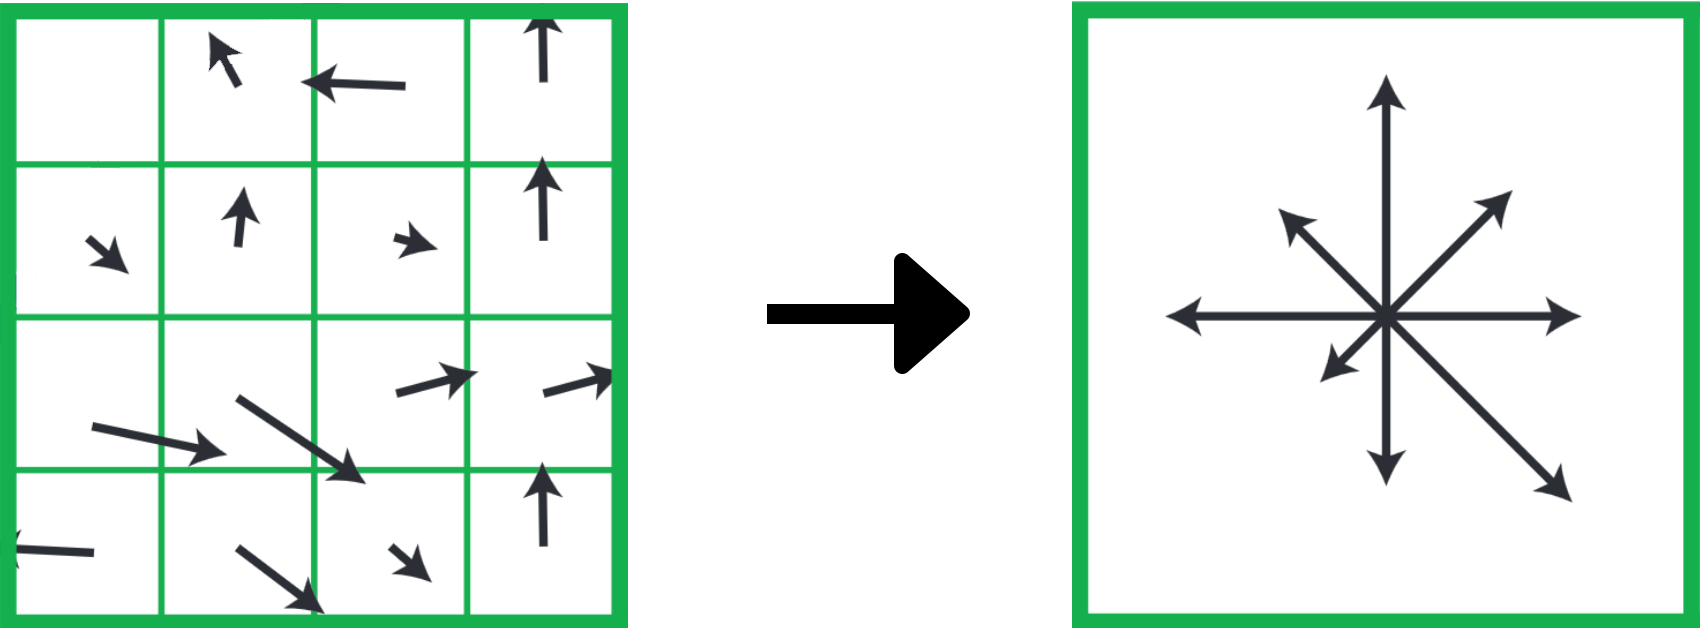
\includegraphics[scale=0.2]{descriptor_histogram_2.png}
                                    \end{center}
                                    Jelen esetben ez egy 8 irányú hisztogram lesz, tehát az egyes csoportok a hisztogramon belül egy 45 fokos szögtartományt fednek le a 360 fokos térből.\\
                                    \begin{center}
                                        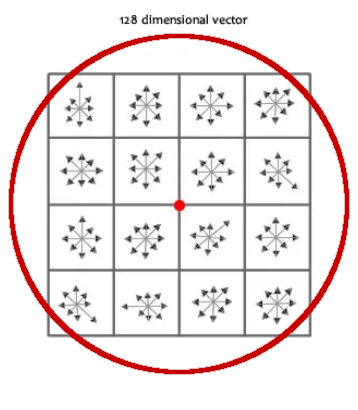
\includegraphics[scale=0.5]{descriptor_weighted.png}
                                    \end{center}
                                    A 16 darab 4x4-es cella hisztogramját végül sorba rendezzük, így kapva egy 128 elemű vektort, amely egy adott kulcspont deszkriptoraként/leírójaként szolgál.\\
                                    A jelenlegi eredmény globális megvilágításváltozásra nem érzékeny, ha a megvilágításváltozás azonos mértékben érinti az összes képpontot, ugyanis a gradiens számolása a pixelek intenzitásának a különbségéből történik. Azonban a nem lináris, lokális megvilágításváltozás hatására lehetnek területek, amelyeket a változás nagyobb mértékben érint, így a gradiensük magnitúdója is nagyobb lesz. Hogy ezen nagy magnitúdójú gradienseknek ne legyen túl nagy befolyása, tovább dolgozzuk őket:
                                    \begin{enumerate}
                                        \item A leíró vektort normalizáljuk:
                                            \[\|d \|_2 = \sqrt{ \sum_{i=1}^{128} d_i^2 }\]
                                            \[d'_i = \frac{d_i}{\|d\|_2} \text{, ahol} \quad i = 1, 2, \dots, 128\]
                                            ahol $\|d \|_2$ a vektor normája, $d'_i$ a vektor egy normalizált komponense.
                                        \item A komponensek küszöbölése: 
                                            \[d''_i = \begin{cases}0.2 & \text{ha } d'_i > 0.2 \\d'_i & \text{ha } d'_i \leq 0.2\end{cases}\]
                                        \item Újabb normalizálás:
                                            \[\|d''\|_2 = \sqrt{ \sum_{i=1}^{128} (d''_i)^2 }\]
                                            \[d'''_i = \frac{d''_i}{\|d''\|_2} \text{, ahol} \quad i = 1, 2, \dots, 128\]
                                            ahol $\|d'' \|_2$ a vektor normája, $d'''_i$ a vektor egy normalizált komponense.
                                    \end{enumerate}
                                    \item \textbf{Kulcspontok megfeleltetése}. A pontmegfeleltetéshez ezek után rendelkezésre áll egy adatbázisnyi kulcspont leíró. Első lépésként megkeressük azt a kulcspontot, amelynek leíró vektora a második képen a legkisebb euklideszi távolságra van a vizsgált kulcspont leíró vektorától. Ezzel a megoldással önmagában az a probléma, hogy a vizsgált ponthoz legközelebb eső szomszéd, nem bizos, hogy a vizsgált pont tényleges párja. Az is lehetséges, hogy az adott pontnak nincs is párja, mert az eleve egy adott képre specifikus zajból adódott vagy esetleg a tényleges párja nem is látszódik a második képen. Ennek kiküszöbölésére a megoldás, hogy összehasonlítjuk a legközelebbi szomszéd és a második legközelebbi szomszéd távolságát. A második legközelebbi szomszéd a vizsgált kulcsponthoz legközelebb eső olyan kulcspont, amely nem a vizsgált kulcsponthoz tartozik (tehát egy szándékos rossz párosítást csinálunk). A helyes pontmegfeleltetések közötti távolságnak jelentősen kisebbnek kell lennie, mint a helytelen pontmegfeleltetések közötti távolságnak. Tehát hamis egyezések esetén valószínűleg számos más hamis egyezés lesz hasonló távolságon belül. (Azaz ezzel kiszűrhetők a könnyen félreérthető pontok. Azt hiszem).\\
                                    Jelen esetben minden olyan megfeleltetést eldobunk ahol a távolságok aránya nagyobb, mint 0.8:
                                    \[\text{A megfeleltetés jó, ha } \frac{\textit{legközelebbi szomszéd}}{\textit{2.legközelebbi szomszéd}} <= 0.8\]
                            \end{enumerate}

                    \item \textit{imshow(image, InitialMagnification = value)} = a meghatározott kép megjelenítése \textit{value}\%-os megnagyításban.
                    \item \textit{hold on} = a következőkben végrehajtott grafikus (pl.: grafikonok kirajzolása, stb.) parancsokat a legutolsó, aktuális ábrára fogja rárajzolni.
                    \item \textit{plot} = létrehoz kétdimenziós grafikont.
                    \item \textit{selectStrongest(featurePoints, N)} = visszaadja az \textit{N} legerősebb (talán ez az intenzitások különbségének nagyságát jelenti) jellemzőpontot (nálunk sarokpontok lesznek) a megadott \textit{featurePoints} változóból.
                    \item \textit{tracker = vision.PointTracker(MaxBidirectionalError=value1, NumPyramidLevels=value2)} = létrehoz egy Kanade-Lucas-Tomasi (KLT) algoritmus szerint működő pontkövető objektumot.\\
                    A KLT algoritmus kifejezetten jól működik olyan objektumok követésére, amely nem változtat alakot, valamint egyedi és részletes textúrával rendelkezik. A KLT algoritmus a Lucas-Kanade (LK) optikai áramlás becslés algoritmuson alapul. Az optikai áramlás az objetumok egy látszólagos/vizuális elmozdulása (nem feltétlenül egyezik meg a valós elmozdulással). Általános feltételezése, hogy egy objektum megfigyelt pixeleinek intenzitása elmozdulástól függetlenül állandó:
                    \[I(x,y,t) = I(x + u,y + v,t + 1)\]
                    Ahol:
                    \begin{itemize}
                        \item \textit{I(x,y,t)} = \textit{(x,y)} pozíción lévő pixel intenzitása \textit{t} időben
                        \item \textit{u} = elmozdulás az x tengelyen
                        \item \textit{v} = elmozdulás az y tengelyen
                    \end{itemize}

                    Ebből kifejezhető az optikai áramlás egyenlete Taylor sort alkalmazva:
                    \[I(x + u,y + v,t + 1) \approx I(x,y,t) + I_xu + I_yv + I_t\]
                    \[I(x + u,y + v,t + 1) - I(x,y,t) = I_xu + I_yv + I_t\]
                    \[0 \approx I_xu + I_yv + I_t\]
                    Ahol:
                    \begin{itemize}
                        \item \textit{$I_xu$} = az intenzitás változása az x tengelyen.
                        \item \textit{$I_yv$} = az intenzitás változása az y tengelyen.
                        \item \textit{$I_t$} = az intentizás idő szerinti változása.
                    \end{itemize}
                    Tehát, ha az \textit{u} és \textit{v} elmozdulások helyesen vannak meghatározva, akkor az intenzitások különbsége megközelítőleg 0. Azonban \textit{u} és \textit{v} ismeretlenek és meghatározásukat nehezíti a \textbf{nyílás/rekesz/apertúra probléma (aperture problem)}, azaz amikor a tényleges mozgást egy kicsi rekeszen keresztül figyelve próbáljuk meghatározni. Egy objektum tényleges elmozdulásának kiszámítása nehéz, ha csak egy kis területet látunk belőle a résen keresztül.\\
                    A Lucas-Kanade algoritmus feltételezi, hogy az optikai áramlás (\textit{u} és \textit{v}) konstans és a képen textúrázott tárgyak láthatók. A megfigyelt pixel kezdeti intenzitása \textit{a}, valamint a rés mögött látható tárgy elmozdítása után észlelt pixel intenzitása \textit{b}. Ezek különbsége \textit{(b - a)}, azaz az időbeli intenzitáskülönbség \textit{$I_t(x,y)$}. A \textit{(x,y)} pozíción megfigyelt pixel intenzitásváltozás \textit{$I_x(x,y)$} az x tengelyen, valamint \textit{$I_y(x,y)$} az y tengelyen. Az x tengelyen történő \textit{u} mértékű és az y tengelyen történő \textit{v} mértékű elmozdulás esetén a pixel intenzitása:
                    \[I_x(x,y)u + I_y(x,y)v = -I_t(x,y)\]
                    Nem tudom miért negatív az $I_t$ :(\\\\
                    Az algoritmus helyes működéséhez nem elegendő egyetlen pixelt nézni, így ezt ki kell terjeszteni egy pixelszomszédságra. Egy 3x3 szomszédság esetén az egyenlet:
                    \[I_x(x + \Delta x, y + \Delta y)u + I_y(x + \Delta x, y + \Delta y)v = -I_t(x + \Delta x, y + \Delta y)\] ahol $\Delta x$ = -1,0,1 (a három szomszédos pixel az x tengelyen), $\Delta y$ = -1,0,1 (a három szomszédos pixel az y tengelyen)
                    Tömör formában a képlet:
                    \[S\begin{bmatrix} u \\ v \end{bmatrix} = \overset{\rightarrow}{t}\]
                    Ahol:
                    \begin{itemize}
                        \item \textit{S} = 9x2 mátrix amely tartalmazza: $[I_x(x + \Delta x, y + \Delta y),  I_y(x + \Delta x, y + \Delta y]$.
                        \item \textit{$\overset{\rightarrow}{t}$} = vektor amely tartalmazza: $-I_t(x + \Delta x, y + \Delta y)$.
                    \end{itemize}
                    Ezen két ismeretlenes egyenlet megoldása a legkisebb négyzetek módszerével történik, amihez megszorozzuk az egyenletet $S^{T}$ (én sem értem miért):
                    \[S^{T}S\begin{bmatrix}u \\ v\end{bmatrix} = S^{T}\overset{\rightarrow}{t}\]
                    Ebből $\begin{bmatrix}u \\ v\end{bmatrix}$ kifejezve:
                    \[\begin{bmatrix}u \\ v\end{bmatrix} = (S^{T}S)^{-1}S^{T}\overset{\rightarrow}{t}\]
                    Röviden (ha jól fogtam fel) a Lucas-Kanade optikai áramlás becslés algoritmusa a képkockák közötti mozgást próbálja nyomon követni. Ehhez két képkockán kiválaszt egy pixelszomszédságot és azok térbeli elmozdulását elemzi. Ezután kiszámolja a pixelértékek intenzitásváltozását, amelyből próbálja kiszámolni az objektum tényleges elmozdulását. Gyorsan mozgó vagy nem ritkásan textúrázott objektumok esetén nem megbízható.\\
                    A tényleges pontmegfeleltetést a Kanade-Lucas-Tomasi (KLT) algoritmus végzi, amelyből a MATLAB vision.PointTracker függvény a pyramid KLT továbbfejlesztett verziót használja. Először minden kiválasztott jellemzőponthoz egy kis ablakot/apertúrát illeszt. A következő lépésben létrehoz egy kép piramist: a kiinduló képből több szintet hoz létre, ahol az alsó szinten található a teljes (eredeti) felbontású kép, a piramis teteje felé haladva a vizsgált kép egyre kisebb felbontású verziója fog szerepelni. Ezután kiszámolja a kiválasztott pixelek elmozdulás vektorait a piramis legfelső szintjétől kezdve, az előbb tárgyalt Lucas-Kanade optikai áramlás becslés algoritmusát felhasználva. A becsült mozgásokat használva finomítja a jellemzőpontok pozícióit a következő alacsonyabban elhelyezkedő, magasabb felbontású piramisszinten. Ezt addig folytatja, amíg el nem éri a legalsó szintet. A piramisos módszer előnye, hogy az alacsonyabb felbontású képeken végzett kezdeti nyomkövetés javítja a teljes nyomkövetési pontosságot és akár nagyobb távolságok követését is lehetővé teszi.\\
                    A \textit{vision.PointTracker} függvényhívásnál használt két argumentum:
                    \begin{itemize}
                        \item \textit{MaxBidirectionalError} = a funkció lényege, hogy az épp vizsgált pontot az első képről követi a második képre, majd ugyanazon pontot követi visszafelé a második képről az első képre. Ezután kiszámolja a vizsgált pont eredeti és a visszakövetés utáni, új pozíciója közötti különbséget (az első képen). Ha ez az érték nagyobb, mint az függvénynek átadott \textit{MaxBidirectionalError} érték, akkor az adott pont érvénytelen. Hatékony módszer a nem megbízhatóan követhető pontok kiküszöbölésére. Az ajánlott érték 0 és 3 pixel között van.
                        \item \textit{NumPyramidLevels} = a képpiramis szintjeinek számát határozza meg. A nagyobb érték lehetővé teszi a nagyobb elmozdulások követését, viszont lassabb futási időt eredményez. Az ajánlott érték 1 és 4 között van.
                    \end{itemize}
                    \item \textit{imagePoints1 = imagePoints1.Location} = a sarokpont objektumok pozícióinak kiolvasása.
                    \item \textit{initialize(pointTracker, points, image1)} = inicializálja az első argumentumként kapott pontkövető objektumot, inicializálja a második argumentumként kapott követendő pontokat, valamint beállítja az utolsó argumentumként kapott képet a kezdeti képkockának.
                    \item \textit{[returnValue1, returnValue2] = step(tracker, image2)} = a \textit{step} függvény indítja el az első argumentumként kapott pontkövető objektumot. A függvény második argumentum a második képkocka, amelyen el kell végeznie a pontkövetést az objektumnak. Az első visszatérési érték a korábban meghatározott jellemzőpontok koordinátái a második képkockán. A második visszatérési érték egy logikai indexvektor, amely azt jelzi, hogy mely pontokat sikerült nyomon követni. A megbízhatóan követhető pontok \textit{true}, míg ellenkező esetben \textit{false} értéket kapnak.
                    \item \textit{matchedPoints = imagePoints(validIdx, :)} = a megbízhatóan követhető pontok lementése. Az \textit{imagePoints} egy mátrix, melynek sorai tartalmazzák a jellemzőpontokat, két oszlopai pedig a jellemzőpontok x és y koordinátáit. A \textit{imagePoints(validIdx, :)} rész egy mátrix címzés, amely visszaadja mátrix azon sorait ahol \textit{validIdx} = \textit{1} vagy \textit{true}, valamint a mátrix összes oszlopát (: jelentése összes index).
                    \item \textit{showMatchedFeatures(image1, image2, matchedPoints1, matchedPoints2)} = a pontmegfeleltetés eredményének kirajzolása. A két agumentumként kapott kép színkódolást kap, valamint a másik két, argumentumként kapott jellemzőpontok is kirajzolódnak és egy vonallal lesznek összekötve a hozzájuk tartozó párjukkal.
                    \item \textit{[returnValue1, returnValue2] = estimateEssentialMatrix(matchedPoints1, matchedPoints2, intrinsics)} = az esszenciális mátrix becslése egy képpár megfeleltetett pontjaiból.\\
                    Az esszenciális mátrix két kamera közötti mozgást kapcsolja össze, megfeleltetett pontpárok közötti geometriai kapcsolatok leírásával. Tehát a különböző szögből készült képekhez használt kamerák relatív helyzetét és orientációját segít meghatározni, \textbf{ha} ismertek a kamera paraméterek (amiket a kamera kalibrációjakor kapunk meg).\\
                    Az esszenciális mátrix egy 3x3 szerkezetű, homogén, 2-es rangú mátrix, amely az alábbi alapján írja le a két képkocka közötti kapcsolatot (\textit{koplanaritási egyenlet}):
                    \[x_1^TEx_2 = 0\]
                    Az $x_1$ egy adott pont homogén koordinátája az első képen, míg az $x_2$ ugyanazon pont homogén koordinátája a második képen (mindkét esetben a kamera koordináta rendszerében, nem pedig pixel koordináta rendszerben):
                    \[x_1 = \begin{bmatrix}x_1\\y_1\\1\end{bmatrix}, x_2 = \begin{bmatrix}x_2\\y_2\\1\end{bmatrix}\]
                    A két képpont kapcsolatát leíró egyenlőség szerint, ha a két képpont ugyanazon pontot írják le, akkor az esszenciális mátrix ($E$) segítségével kifejezhető a köztük lévő kapcsolat. A képlet szétbontva:\\
                    \[\begin{bmatrix}x_1&y_1&1\end{bmatrix}\begin{bmatrix}E_{11}&E_{12}&E_{13}\\E_{21}&E_{22}&E_{23}\\E_{31}&E_{32}&E_{33}\end{bmatrix}\begin{bmatrix}x_2\\y_2\\1\end{bmatrix} = 0\]
                        \hspace{3cm} $\overset{\uparrow}{ismert}$ \hspace{1cm} $\overset{\uparrow}{ismeretlen}$ \hspace{0.1cm} $\overset{\uparrow}{ismert}$\\
                    Ha elvégezzük az ismert elemek szorzatát, majd szétválasztjuk az ismeretlen az ismert részektől:
                    \[A\begin{bmatrix}E_{11}\\\vdots\\E_{33}\end{bmatrix} = 0\]
                    Ezt szinguláris érték felbontással végezhetjük el, megkapva az esszenciális mátrixot. Ezt a módszert 8 pont algoritmusnak hívják, amely minimum 8 pontpárt és normalizált koordinátákat követel meg.
                    Az esszenciális mátrix két alapvető elemből áll:
                    \[E = [t]_xR\]
                    Ahol:
                    \begin{itemize}
                        \item \textit{R} = egy ortogonális 3x3-as rotációs mátrix amely a kamerák közötti forgást írja le: $R = \begin{bmatrix}r_{11}&r_{12}&r_{13}\\r_{21}&r_{22}&r_{23}\\r_{31}&r_{32}&r_{33}\end{bmatrix}$
                        \item \textit{[$t_x$]} = a \textit{t} egy transzlációs vektor, amely a kamera két pozíciójának közötti eltolást írja le: $t = \begin{bmatrix}t_x\\t_y\\t_z\end{bmatrix}$. \textit{[$t_x$]} = a transzlációs vektor ferde mátrixa (\textit{skew-symmetric matrix}, én sem tudom mi az), amely biztosítja, hogy a vektorok közötti keresztszorzat mátrixművelettel leírható legyen: $[t]_x = \begin{bmatrix}0&-t_z&t_y\\t_z&0&-t_x\\-t_y&t_x&0\end{bmatrix}$\\
                    \end{itemize}
                    Ez a rész valószínűleg erősen hiányos, de nem teljesen értem, hogy hogyan történik az esszenciális mátrix becslése.\\
                    A második visszatérési érték, az \textit{epipolarInliers} megadja, hogy a megfeleltetett pontok mennyire esnek közel az epipoláris síkhoz. (Ha jól értelmeztem) az epipoláris sík magyarázata:\\
                    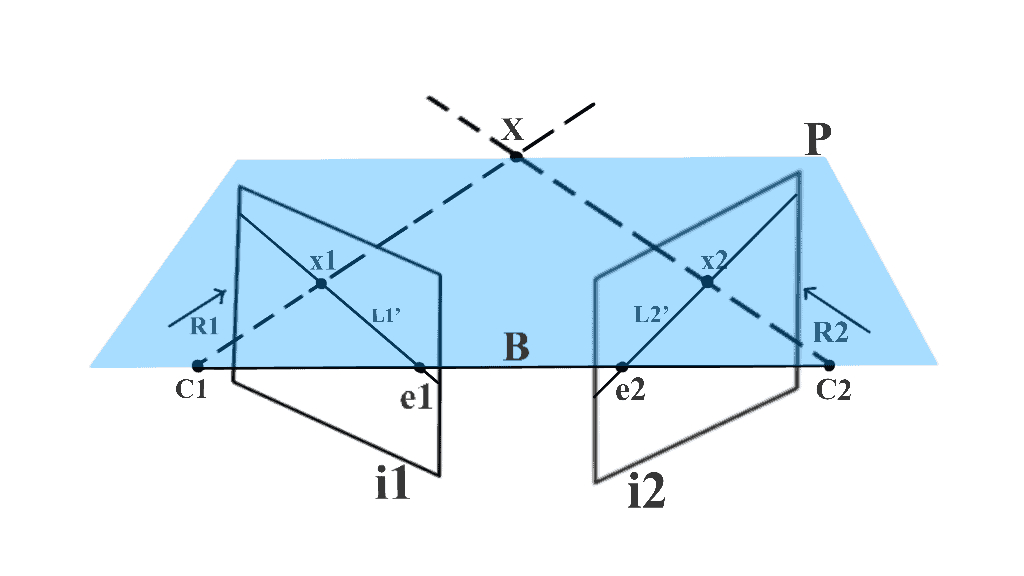
\includegraphics[scale=0.4]{epipolar_line.jpg}
                    Az X pontról készítünk egy-egy képet két különböző szemszögből (a kamera középpontja az első pozícióban $C_1$, míg a második pozícióban lévő kamera középpontja $C_2$). Az első képen az X pont $x_1$ pontban, míg a második képen $x_2$ pontban lett megörökítve. Ha húzunk egy vonalat a $C_1$ középpontból a képen szereplő $x_1$ ponton túl, a vonal át fog haladni a lefényképezett X ponton, azaz az első képen $x_1$ pont a $C_1$ kameraközéppont és a lefényképezett X pont közé húzott vonalon helyezkedik el (ez a vonal az $R_1$). Ha ez a vonal látható lenne, akkor a második képen látható részlete lenne a második képhez tartozó epipoláris vonal ($L_2$). Ahogy az első képen az $x_1$ az $R_1$ vonalon helyezkedik el, úgy a második képen az $x_2$ pontnak is az $L_2$ epipoláris vonalon kell elhelyezkednie.\\
                    A MATLAB \textit{estimateEssentialMatrix} függvény egy \textit{MSAC} elnevezésű algoritmust használ, hogy eldöntse mely pontok outlierek (az epipoláris síktól messze találhatóak) és melyek az inlierek (az epipoláris síkhoz közel találhatóak). Mivel a megfeleltetett képpontoknak az epipoláris síkon kellene elhelyezkedniük, az outlierek rosszul lettek párosítva a pontmegfeleltetés során, így ezeket kiszűrjük.
                    \item \textit{inlierPoints = matchedPoints(epipolarInliers, :)} = lementsük az epipoláris vonalhoz közel eső (tehát a valószínűleg helyesen párosított) pontokat.
                    \item \textit{estrelpose(essentialMatrix,intrinsics,inlierPoints1,inlierPoints2)} = kiszámítja a második kamera relatív pozícióját az elsőhöz képest az esszenciális mátrixból kinyert rotációs mátrix és transzlációs vektor alapján. Nem találtam meg, hogy pontosan hogyan teszi ezt :(
                    \item \textit{camProjection = cameraProjection(intrinsics,tform)} = a visszatérési értéke egy kamera vetítési mátrix. Homogén koordinátával rendelkező, 3D pontok képre való vetítésére szolgál az argumentumként kapott \textit{tform} transzformáció szerint, valamint a kamera belső paramétereit is figyelembe véve.\\
                    A vetítési mátrix egy 3x4 szerkezetű mátrix, amely leírja a kamera valóvilágbéli, 3D pontok leképezését 2D pontokra a képsíkra/elkészült képre:
                    \[x = PX\]
                    Ahol:
                    \begin{itemize}
                        \item \textit{x} = 2D képpont = $\begin{bmatrix}X\\Y\\Z\end{bmatrix}$
                            \item \textit{P} = kamera mátrix = $K\begin{bmatrix}R|t\end{bmatrix}$, ahol \textit{K} = a kamera belső paraméterei, \textit{R} = rotációs mátrix, \textit{t} = transzlációs mátrix.
                            \item \textit{X} = 3D pont a valóvilágban = $\begin{bmatrix}X\\Y\\Z\\1\end{bmatrix}$
                    \end{itemize}
                    Az alkalmazott merev transzformáció (\textit{rigidtform3d}) egy olyan transzformáció, amelybe beletartozik a forgatás és eltolás, de nem változtatja meg az objektum méretét és formáját. Ha nem adunk meg semmilyen argumentumot, akkor a \textit{rigidtform3d} egy identitás transzformációt hajt végre, amely semmilyen módon nem változtatja meg az objektumot a leképezés során (forgatást és eltolást is beleértve). Mivel az első kamera a referenciapontunk (tehát az első kamera az origón található), ezért csak egységtranszformációt hajtunk végre.
                    A kamera mátrix kiszámítása a meghatározott transzformációval:
                    \[P = K\begin{bmatrix}rigidtform3d.R|rigidtform3d.t\end{bmatrix}\]
                   
                    A mátrix tartalmazza a képre vetített 3D pontokat homogén koordinátákban.\\
                    A második kamera esetében az első kamera szerinti relatív elhelyezkedést és orientációt (\textit{relPose}) átadjuk a \textit{pose2extr} függvénynek, amely visszaadja a kamera külső paramétereit (extrinsic mátrix). A kamera külső paraméterei azt mutatják meg, hogyan kell a kamera koordináta-rendszeréből a világ koordináta-rendszerébe végrehajtani a transzformációt. Ez azt jelenti, hogy ha van egy pont a kamera koordináta-rendszerében, akkor a \textit{pose2extr} által visszaadott extrinsic mátrix segítségével átalakíthatjuk ezt a pontot a világ koordináta-rendszerébe. Innentől fogva a \textit{cameraProjection} függvény a belső és külső paramétereket felhasználva leírja a második kamerához tartozó kamera vetítési mátrixot. (Nem tudom mennyire helyes ez a bekezdés).
                    \item \textit{triangulate(matchedPoints1, matchedPoints2, camProjection1, camProjection2)} = Az argumentumként kapott pontpárok és kamera vetítési mátrixok segítségével háromszögelést végez. Visszatérési értéke a megfeleltetett pontpárok világkoordináta-rendszerbeli koordinátái.\\
                    Az előző pontokban említettük, hogy a kamera mátrix megadja a 3D pont képsíkra történő 2D leírását:
                    \[x = PX\]
                Mivel ismert az \textit{x} és a \textit{P} elméletben ebből az X könnyen meghatározható:\\
                    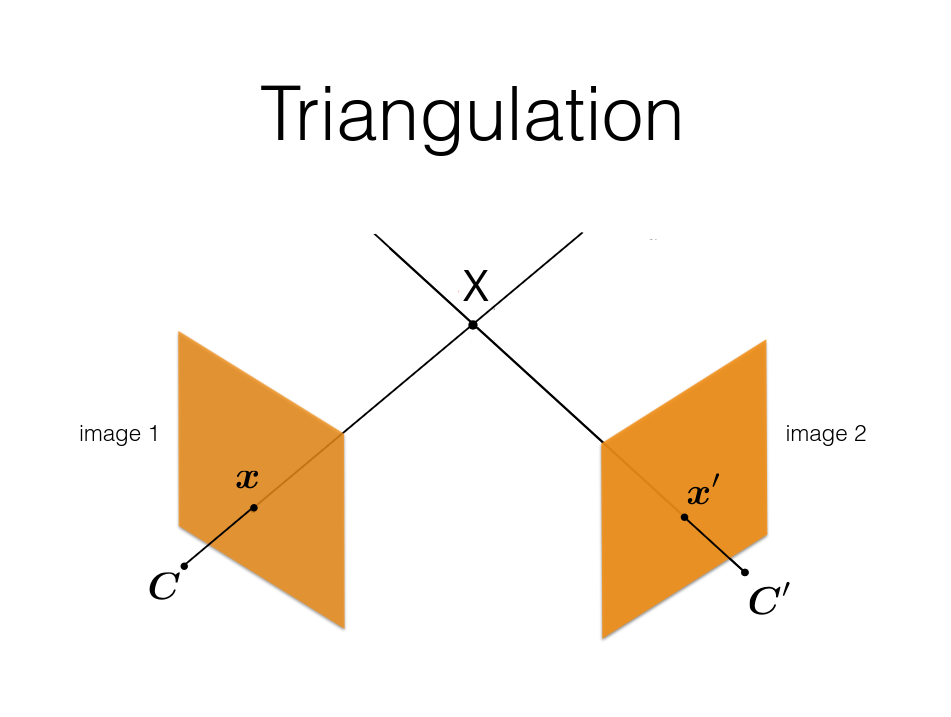
\includegraphics[scale=0.4]{triangulation.png}
                    \begin{itemize}
                        \item \textit{C} = az első kamera középpontja.
                        \item \textit{C'} = a második kamera középpontja.
                        \item \textit{x} = az első kamera \textit{X} objektumról készített leképezése az első képsíkra.
                        \item \textit{x'} = a második kamera \textit{X} objektumról készített leképezése a második képsíkra.
                        \item \textit{X} = az eredeti 3D objektum.
                    \end{itemize}
                    Elméletben tehát ha húzunk egy vetítősugarat az első kamera középpontjából kezdve, át az \textit{x} ponton, valamint húzunk még egy vetítősugarat a második kamera középpontjától kezdve, át az \textit{x'} ponton, a két egyenes metszéspontja meg kell határoznia \textit{X} pontot. A probléma, hogy ehhez tökéletes mérések kellenek, a valóságban viszont a különböző zajok és mérési pontatlanságok miatt  a két vetítősugár nem fogja metszeni egymást. Ennek következtében a valóságban csak közelítő eredményt keresünk. A háromszögelés lináris megoldása: \\
                    Szétbontjuk az alábbi egyenletet:\\
                    \[x = PX\]
                    \[\begin{bmatrix}x\\y\\z\end{bmatrix} = 
                        \begin{bmatrix}
                        p_{11} & p_{12} & p_{13} & p_{14} \\
                        p_{21} & p_{22} & p_{23} & p_{24} \\
                        p_{31} & p_{32} & p_{33} & p_{34}
                        \end{bmatrix}
                        \begin{bmatrix}X\\Y\\Z\\1\end{bmatrix}\]
                        Vesszük a P mátrix sorait és transzponáljuk:
                        \[\begin{bmatrix}x\\y\\z\end{bmatrix} = 
                        \begin{bmatrix}
                        \xdash & p_{1}^T & \xdash \\
                        \xdash & p_{2}^T & \xdash \\
                        \xdash & p_{3}^T & \xdash
                        \end{bmatrix}
                        \begin{bmatrix}\ydash\\X\\\ydash\end{bmatrix}\]
                        A mátrix egyes sorait szorozzuk az \textit{X} vektorral:
                        \[\begin{bmatrix}x\\y\\z\end{bmatrix} =
                        \begin{bmatrix}
                        p_{1}^TX\\
                        p_{2}^TX\\
                        p_{3}^TX
                        \end{bmatrix}\]
                        Vesszük az egyenlőség két oldalának keresztszorzatát:
                        \[\begin{bmatrix}x\\y\\z\end{bmatrix} \times \begin{bmatrix}
                        p_{1}^TX\\
                        p_{2}^TX\\
                        p_{3}^TX
                        \end{bmatrix} = 0\]
                        (\textit{Két párhuzamos vektor keresztszorzata 0. Keresztszorzatot az alábbi minta szerint végzünk:
                        \[a \times b = \begin{bmatrix} 
                            a_2 b_3 - a_3 b_2 \\ 
                            a_3 b_1 - a_1 b_3 \\ 
                            a_1 b_2 - a_2 b_1 
                            \end{bmatrix}
                        \]})
                        \[\begin{bmatrix}
                        yp_3^TX - p_2^TX \\
                        p_1^TX - xp_3^TX \\
                        xp_2^TX - yp_1^TX
                        \end{bmatrix} = 0\]
                        A harmadik sor az első két sor kombinációja (az első sor \textit{x}-szer, és a második sor \textit{y}-szor), az a sor jelenleg nem jelentős, így azt elhagyjuk.\\
                        Az eddigi eljárást megcsináljuk mindkét kamera esetében:
                        \[\begin{bmatrix}
                        yp_3^{T}X - p_2^{T}X \\
                        p_1^{T}X - xp_3^{T}X \\
                        \end{bmatrix} = 0, 
                        \begin{bmatrix}
                        y^{'}p_3^{'T}X - p_2^{'T}X \\
                        p_1^{'T} - x'p_3^{'T}X \\
                        \end{bmatrix} = 0\]
                        A két mátrixot összeillesztjük és kiemeljük az \textit{X}-et:
                        \[\begin{bmatrix}
                        yp_3^{T} - p_2^{T} \\
                        p_1^{T} - xp_3^{T} \\
                        y^{'}p_3^{'T} - p_2^{'T} \\
                        p_1^{'T} - x'p_3^{'T}
                        \end{bmatrix}X = 0\]
                        A mátrixot egy \textit{A}-val jelöljük:
                        \[AX = 0\]
                        Ez az egyenlőség pedig szinguláris értékek felbontásával (SVD) oldható, megkapva a pont közelítő, 3D koordinátáját.
                        \item \textit{numPixels = size(var, dim1) * size(var, dim2)} = a \textit{size} függvény visszatérési értéke a \textit{var} változó mérete a meghatározott \textit{dim1} dimenzióban (\textit{1} = sorok száma, \textit{2} = oszlopok száma). A mi példánkban az egyenlettel lekérjük a kép magasságát és szélességét, ezek szorzatával pedig kiszámítsuk a kép pixeleinek számát.
                        \item \textit{allColors = reshape(I1, [numPixels, 3])} = a megadott képet átalakítjuk egy tömbbé, amelynek minden sora a kép egy pixele, az oszlopai pedig az adott sorban található pixel RGB értékét adja meg.
                        \item \textit{colorIdx = sub2ind([size(I1, 1), size(I1, 2)], round(matchedPoints1(:,2)),round(matchedPoints1(:, 1)))} = A megfeleltetett pontok indexeinek kiolvasása. Az indexeket subscript (sor és oszlop indexek) típusból lineáris indexszé (az index egy darab szám, amely az oszlopok mentén haladva a legelső elemtől kezdődik) alakítjuk.
                        \item \textit{color = allColors(colorIdx, :)} = kiolvassuk a megfeleltetett pontok színeit az indexvektor segítségével.
                        \item \textit{pointCloud(xyzPoints, colors)} = meghatározott színekkel létrehozza a pontfelhő objektumot.
                        \item \textit{figure\\
                                      plotCamera(Size=cameraSize, Color="r", Label="1", Opacity=0);\\
                                      hold on\\
                                      grid on\\
                                      plotCamera(AbsolutePose=relPose, Size=cameraSize,Color="b", Label="2", Opacity=0)} = kirajzoljuk az első kamerát az origóba piros színnel, majd pedig a második kamerát kék színnel az első kamera pozíciójától a kiszámolt relatív pozícióba.
                \end{enumerate}

    \chapter{Forrás}
        \begin{itemize}
            \item \url{https://www.mathworks.com/help/vision/ug/structure-from-motion-from-two-}\\\url{views.html}
            \item \url{https://www.mathworks.com/help/vision/ref/undistortimage.html?s_tid=doc_ta}
            \item \url{https://www.mathworks.com/help/visionhdl/ug/image-undistort.html}
            \item \url{https://e-learning.ujs.sk/pluginfile.php/23441/mod_resource/content/1/01-ProjektivKamera.pdf}
            \item \url{https://www.mathworks.com/help/vision/ref/detectmineigenfeatures.html}
            \item \url{https://aishack.in/tutorials/features/}
            \item \url{https://aishack.in/tutorials/harris-corner-detector/}
            \item \url{https://aishack.in/tutorials/shitomasi-corner-detector/}
            \item \url{https://docs.opencv.org/3.4/dc/d0d/tutorial_py_features_harris.html}
            \item \url{https://www.mathworks.com/help/vision/ref/vision.pointtracker-system-object.html}
            \item \url{https://lorenzopeppoloni.com/lkttracker/}
            \item \url{https://www.baeldung.com/cs/optical-flow-lucas-kanade-method}
            \item \url{https://www.inf.u-szeged.hu/~kato/teaching/IpariKepfeldolgozas/08-Motion.pdf}
            \item \url{http://www.inf.fu-berlin.de/inst/ag-ki/rojas_home/documents/tutorials/Lucas-Kanade2.pdf}
            \item \url{https://link.springer.com/chapter/10.1007/978-3-319-29451-3_29}
            \item \url{https://www.mathworks.com/help/matlab/ref/step.html}
            \item \url{https://www.mathworks.com/help/vision/ref/showmatchedfeatures.html}
            \item \url{https://www.baeldung.com/cs/fundamental-matrix-vs-essential-matrix}
            \item \url{https://e-learning.ujs.sk/pluginfile.php/23450/mod_resource/content/1/05-SztereoKamera.pdf}
            \item \url{https://learnopencv.com/introduction-to-epipolar-geometry-and-stereo-vision/}
            \item \url{https://www.mathworks.com/help/vision/ref/estrelpose.html}
            \item \url{https://www.mathworks.com/help/vision/ref/cameraprojection.html}
            \item \url{https://ksimek.github.io/2012/08/14/decompose/}
            \item \url{https://www.cs.cmu.edu/~16385/s17/Slides/11.1_Camera_matrix.pdf}
            \item \url{https://www.mathworks.com/help/images/ref/rigidtform3d.html}
            \item \url{https://www.storyofmathematics.com/rigid-transformation/}
            \item \url{https://staff.fnwi.uva.nl/r.vandenboomgaard/ComputerVision/LectureNotes/CV/StereoVision/triangulation.html}
            \item \url{https://e-learning.ujs.sk/pluginfile.php/23450/mod_resource/content/1/05-SztereoKamera.pdf}
        \textbf{SIFT}
            \item \url{https://www.mathworks.com/help/vision/ref/detectsiftfeatures.html}
            \item \url{https://docs.opencv.org/3.4/da/df5/tutorial_py_sift_intro.html}
            \item \url{https://www.cs.ubc.ca/~lowe/papers/ijcv04.pdf}
            \item \url{https://www.geeksforgeeks.org/describe-the-concept-of-scale-invariant-feature-transform-sift/}
        \end{itemize}
\end{document}
